%\documentclass[9pt]{scrartcl}
\documentclass[a4paper]{article}
\usepackage[]{amsmath}
\usepackage{tikz}
\usetikzlibrary{positioning}
%\usepackage{helvet}
\usepackage{listings}
\usepackage{geometry}
\usepackage{enumitem}
%\geometry{textheight=\paperheight, noheadfoot, nomarginpar}
\geometry{margin=0.5in}
\usetikzlibrary{positioning,shapes,shadows}
\renewcommand{\familydefault}{\sfdefault}

\tikzstyle{abstract}=[rectangle, draw=black, fill=gray!20, text centered,  text=black, text width=12.5mm]
\tikzstyle{spacestyle}=[rectangle, draw=black, fill=gray!20, text centered,  text=black, text width=50mm]

\lstset{
        language=python,
        basicstyle=\fontencoding{T1}\ttfamily,
        commentstyle=\color{gray},
        keywordstyle=\color{OliveGreen},
        frame=single,
        backgroundcolor=\color{lightlightgray},
        tabsize=2,
        %deletestring=[d]",
        %escapechar=\%,
        numbers=left,
        showstringspaces=false,
}
\usepackage[explicit]{titlesec} 
\titleformat{\section}{\normalfont\Large\bfseries}{}{0em}{#1}
\titleformat{\subsection}{\normalfont\bfseries}{}{0em}{--#1}

\newcommand{\mykey}[2]{%
\begin{tikzpicture} \node (Item) [abstract, minimum size=12.5mm, align=center]
{\vrule height 12pt depth 8pt width 0pt\textbf{#1} \\\vrule height 6pt depth 8pt width 0pt\parbox{1.25cm}{\centering{\fontsize{6pt}{8pt}\selectfont{#2}}}};%
\end{tikzpicture}}


\begin{document}
\begin{center}
\Large{Diagram}
\end{center}
\noindent%


\section {Vector clock diagram}
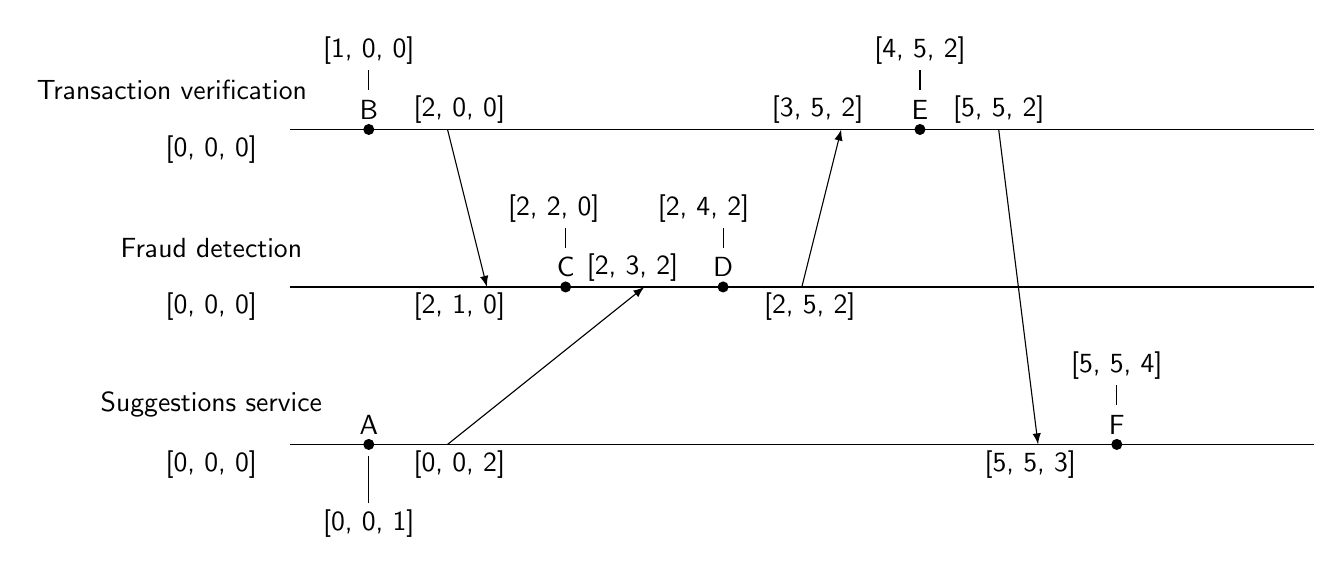
\begin{tikzpicture}

\node at (0, 0.5) {Suggestions service};
\node at (0, -0.25) {[0, 0, 0]};
\node at (0, 2.5) {Fraud detection};
\node at (0, 1.75) {[0, 0, 0]};
\node at (-0.5, 4.5) {Transaction verification};
\node at (0, 3.75) {[0, 0, 0]};

% Draw horizontal lines
\draw (1,0) -- (14,0);
\draw (1,2) -- (14,2);
\draw (1,4) -- (14,4);

%\node at (3, -0.25) {[0, 0, 2]};
%\draw[-latex] (3, 0) -- (4, 2);
%\fill (1.5,0) circle [radius=2pt];
%\node at (1.5,-0.25) {A};

\fill (2, 0) circle [radius=2pt];
\node at (2, 0.25) {A};

\fill (2, 4) circle [radius=2pt];
\node at (2, 4.25) {B};

\draw[-latex] (3, 4) -- (3.5, 2);

\fill (4.5, 2) circle [radius=2pt];
\node at (4.5, 2.25) {C};

\draw[-latex] (3, 0) -- (5.5, 2);

\fill (6.5, 2) circle [radius=2pt];
\node at (6.5, 2.25) {D};

\draw[-latex] (7.5, 2) -- (8, 4);

\fill (9, 4) circle [radius=2pt];
\node at (9, 4.25) {E};

\draw[-latex] (10, 4) -- (10.5, 0);

\fill (11.5, 0) circle [radius=2pt];
\node at (11.5, 0.25) {F};



\node at (2, -1) {[0, 0, 1]};
\draw (2, -0.75) -- (2, -0.15);

\node at (3.15, -0.25) {[0, 0, 2]};

\node at (2, 5) {[1, 0, 0]};
\draw (2, 4.75) -- (2, 4.5);

\node at (3.15, 4.25) {[2, 0, 0]};

\node at (3.15, 1.75) {[2, 1, 0]};

\node at (4.35, 3) {[2, 2, 0]};
\draw (4.5, 2.75) -- (4.5, 2.5);

\node at (5.35, 2.25) {[2, 3, 2]};

\node at (6.25, 3) {[2, 4, 2]};
\draw (6.5, 2.75) -- (6.5, 2.5);

\node at (7.6, 1.75) {[2, 5, 2]};

\node at (7.7, 4.25) {[3, 5, 2]};

\node at (9, 5) {[4, 5, 2]};
\draw (9, 4.75) -- (9, 4.5);

\node at (10, 4.25) {[5, 5, 2]};

\node at (10.4, -0.25) {[5, 5, 3]};

\node at (11.5, 1) {[5, 5, 4]};
\draw (11.5, 0.75) -- (11.5, 0.5);

\end{tikzpicture}

\section{Event legend}
%\renewcommand{\theenumi}{\Alph{enumi}}
\begin{enumerate}[label=\Alph* -]
\item Suggestion service checks that it is able to tokenize the book name
\item Check that name is non-empty
\item Check that name does not contain suspicious characteristics
\item Check that credit card number is not associated with the devil
\item Check that credit card number is not empty
\item Choose book to suggest next
\end{enumerate}

\end{document}